% dimred

\begin{frame}
  \frametitle{Réduction de dimensions - Problème}
  \begin{itemize}
  \item Grand nombre $p$ de variables (centaines ou milliers de variables).
  \item Si $n$ est grand, on parle de \red{big data}.   
  \item Si $p$ est grand par rapport à $n$, on parle de \red{fat data}. 
  \item Réduction de dimensions : trouver pour une matrice de données $X\in \RR^{n\times p}$ une représentation $X \in \RR^{n\times m}$, avec $p\gg m$. 
  \end{itemize}
\end{frame}

\begin{frame}
  \frametitle{Réduction de dimensions - Motivation}
  \begin{itemize}
  \item Visualisation / exploration : une étape importante
  \item Identifier des artefacts
  \item Réduction du coût computationnel
  \item Moins de descripteurs pour de meilleurs algorithmes de prédiction : 
  \begin{itemize}
  	\item moins de paramètres à estimer
  	\item moins de bruit
  	\item moins de dimensions peu informatives
  	\item éviter le fléau de la dimensionalité
  \end{itemize}
  \end{itemize}
\end{frame}

\begin{frame}
  \frametitle{Réduction de dimensions - deux stratégies}
  \begin{itemize}
  	\item \red{Sélection de variables} : éliminer les variables peu utiles
  	\item \red{Extraction de variables} : créer $m$ nouvelles variables à partir des $p$ variables
  \end{itemize}
\end{frame}

\begin{frame}
  \frametitle{Méthode de filtrage}
  \begin{itemize}
  	\item Filtrage non-supervisé (exemple : enlever des variables corrélées )
  	\item Filtrage supervisé : enlever des variables qui ne sont pas statistiquement associées à la variable de sortie
  \end{itemize}
\end{frame}

\begin{frame}
  \frametitle{Méthode de filtrage - limitations}
	\begin{figure}[htb]
	  \centering
	  \includegraphics[width=.6\textwidth]{guyon.pdf}
	%  \source{adapted from \url{https://cs.stanford.edu/people/karpathy/cnnembed/}}
	\end{figure}
  	Des variables corrélées et non-significatives peuvent tout de même être utiles (dans le contexte d'autres variables).
\end{frame}

\begin{frame}
  \frametitle{Méthode de conteneur}
  \begin{itemize}
  	\item Méthode supervisée de sélection de variables. 
  	\item Liée à une méthode de classification : on juge la qualité de la variable par rapport à la performance de classification.
  	\item 2 stratégies : 
  	\begin{itemize}
  		\item \red{Méthode ascendante (forward selection)}: successivement ajouter des variables
  		\item \red{Méthode descendante (backward selection)}: successivement enlever des variables
  	\end{itemize}
  \end{itemize}
\end{frame}

\begin{frame}
  \frametitle{Méthode ascendante}
  \begin{itemize}
  	\item On commence avec un ensemble de variables vide $\fcal = \emptyset$
  	\item A chaque étape, on ajoute la variable qui apporte le meilleur gain en performance de classification.
  	\item On arrête, quand la performance ne s'améliore plus. 
  \end{itemize}
\end{frame}

\begin{frame}
  \frametitle{Méthode descendante}
  \begin{itemize}
  	\item On commence avec l'ensemble de toutes les variables $\fcal$
  	\item A chaque étape, on enlève la variable sans laquelle on obtient la meilleure performance de classification.
  	\item On arrête, quand la performance ne s'améliore plus. 
  \end{itemize}
\end{frame}

\begin{frame}
  \frametitle{Méthode de conteneur - limitations}
  \begin{itemize}
  	\item L'ensemble de variables identifiés dépend du classifieur utilisé (il ne s'agit pas d'un critère général). 
  	\item Méthode gloutonne (greedy method): aucune garantie d'optimalité. 
  \end{itemize}
\end{frame}

\begin{frame}
  \frametitle{Méthodes embarquées}
  \begin{itemize}
  	\item Méthodes de classification avec un mécanisme de sélection de variables
  	\item Exemple : l'utilisation de la norme $L_1$ (valeur absolue).  
  	\item Pour rappel : 
  \end{itemize}
  \begin{center}
    \includegraphics[width=.6\textwidth]{figures/l1reg_geom}  
  \end{center}
\end{frame}

\begin{frame}
  \frametitle{Analyse en composantes principales}
  \begin{itemize}
  	\item Analyse en composantes principales (ACP) (principal component analysis, PCA)
  	\item Méthode non-supervisée (aucune étiquette est utilisée)
  	\item Expression de $X\in \RR^{n\times p}$ dans une base orthonormée, par une transformation linéaire orthogonale.
  	\item Maximisation de la variance.
%  	\item Premier axe : projection de $X$ avec la plus grande variance
%  	\item Deuxième axe : projection de $X$ avec la plus grande variance, orthogonale à la première. 
%  	\item $\ldots$
  \end{itemize}
\end{frame}

\begin{frame}
  \frametitle{Extraction de variables - ACP}
	\begin{figure}[htb]
	  \centering
	  \includegraphics[width=.8\textwidth]{pca.pdf}
	%  \source{adapted from \url{https://cs.stanford.edu/people/karpathy/cnnembed/}}
	\end{figure}
\end{frame}

\begin{frame}
\frametitle{ACP: Méthode 1/3}
  \begin{itemize}
  	\item Première étape : centrer les colonnes de $X \in \RR^{n \times p}$: 
 \begin{equation*}
 x^i_j = \frac{x_j^i - \overline{x}_j}{\sqrt{\frac{1}{n}\sum_{l=1}^n(x_j^l - \overline{x}_j)^2}} 
 \end{equation*}
 	\item La matrice de covariance est donc : $\Sigma = \frac1n X^TX$ 
 	\item On cherche maintenant une direction $\wvec$, pour laquelle la projection de $X$ sur cette direction a une variance maximale. 
 	\item On peut montrer que cette variance maximale est la plus grande valeur propre de $\Sigma$, et que la direction est le vecteur propre correspondant. 
  \end{itemize}
\end{frame}

\begin{frame}
\frametitle{ACP: Méthode 2/3}
  \begin{itemize}
  	\item Si on ordonne les valeurs propres de $\Sigma$ selon leurs tailles, on obtient les composantes principales $cp_2, cp_3, \ldots$ qui remplissent les critères suivants : 
  	\begin{itemize}
  		\item Chaque $cp_i$ est orthogonal à toutes les autres composantes.
  		\item La variance de la projection de $X$ sur $cp_i$ est identique à la valeur propre $i$. 
  	\end{itemize}
  	\item Nous en déduisons : 
  	\begin{itemize}
  		\item Les projections de $X$ sur les composantes principales sont décorrélées. 
  		\item Les composantes principales $cp_i$ contiennent de moins en moins d'information (avec $i$ croissant). 
  	\end{itemize}
  \end{itemize}
\end{frame}

\begin{frame}
\frametitle{ACP: Méthode 3/3}
  \begin{itemize}
  	\item L'ACP nous donne donc une transformation avec : des variables décorrélées, et ordonnées selon l'importance. 
  	\item Typiquement, on choisit un nombre $m$ de composantes principales. Le critère pour $m$ est la variance "expliquée" par le modèle. 
  	\item On peut aussi choisir $m=2$ ou $m=3$ pour la visualisation par exemple.   
  \end{itemize}
\end{frame}

\begin{frame}
\frametitle{ACP: avantages et inconvénients}
  \begin{itemize}
  	\item Avantages : 
  	\begin{itemize}
  		\item non-supervisé
  		\item projections décorrélées 
  		\item simple, méthode linéaire
  	\end{itemize}
  	\item Inconvénients : 
  	\begin{itemize}
  		\item la variance maximale n'est pas identique avec le contenu d'information
  		\item en pratique, les structures locales ne sont pas nécessairement bien préservées 
  	\end{itemize}
  \end{itemize}
\end{frame}

\begin{frame}
\frametitle{t-SNE 1/3}
\begin{itemize}
%	\item Many low dimensional representations: PCA, ICA, $\ldots$
	\item Objectif : représentation des données en basse dimension en respectant les relations locales
	\item Une technique relativement récente  \emph{t-Distributed Stochastic Neighbor Embedding (t-SNE)} (2008)
	\item $\{\xvec_i\}_{0\leq i < N}$ sont les représentations, avec $\xvec \in \RR^p$. 
	\item On définit la probabilité que $x_j$ est voisin de $x_i$, sous condition que la probabilité peut être modélisée par une Gaussienne, centrée dans $x_i$:  
	\begin{equation}
	p_{j|i} = \frac{\exp{\left(-\frac{\|\xvec_i - \xvec_j\|^2}{2 \sigma_i^2}\right)}}{\sum_{k\neq i} \exp{\left(-\frac{\|\xvec_i - \xvec_k\|^2}{2 \sigma_i^2}\right)} }
	\end{equation}
	Le paramètre $\sigma_i$ varie avec l'échantillon $x_i$. 
\end{itemize}
\end{frame}


\begin{frame}
\frametitle{t-SNE 2/3}
\begin{itemize}
	\item On souhaite assigner aux vecteurs $\{\xvec_i\}$ des représentations $\{\widetilde{\xvec_i}\}$ tout en préservant les probabilités de voisinages $q_{j|i}$: 
	\begin{equation*}
	q_{j|i} = \frac{\exp{\left(-\|\widetilde{\xvec_i} - \widetilde{\xvec_j}\|^2\right)}}{\sum_{k\neq i} \exp{\left(-\|\widetilde{\xvec_i} - \widetilde{\xvec_k}\|^2\right)} }
	\end{equation*}
	\item Cela peut être fait par la minimisation de la divergence Kulback-Leibler entre les distributions $P_i$ (distribution de $p_{j|i}$) et $Q_i$ (distribution de $q_{j|i}$): 
	\begin{equation}
		C = \sum_i KL(P_i\|Q_i) = \sum_i \sum_j p_{j|i}\log{\frac{p_{j|i}}{q_{j|i}}}
	\end{equation}
	\item Si $\xvec_i$ and $\xvec_j$ sont proches dans l'espace originale, l'algorithme va essayer de pousser $q_{j|i}$ vers $p_{j|i}$ (pour que le ratio soit 1). 
	\item Si $\xvec_i$ et $\xvec_j$ sont loin dans l'espace d'origine, il n'est pas garanti qu'ils le soient dans l'espace à basse dimension. 
\end{itemize}
\end{frame}

\begin{frame}
\frametitle{t-SNE 3/3}
\begin{itemize}
	\item Les paramètres $\sigma_i$ sont déterminés par l'algorithme
	\item Ils varient selon la densité de voisins, de façon à ce que pour chaque $\xvec_i$ nous avons à peu près le même nombre de voisins. 
	\item L'utilisateur choisit le paramètre \textit{perplexity} qui mesure le nombre effectif de voisins. 
	\item Le problème se réduit à la solution d'un problème d'optimisation $\min_{\widetilde{\xvec_i}} C$ avec la méthode du gradient.
\end{itemize}
\end{frame}

\begin{frame}
\frametitle{t-SNE: avantages et inconvénients}
  \begin{itemize}
  	\item Avantages : 
  	\begin{itemize}
  		\item conserve les structures locales
  		\item permet d'identifier des cluster potentiels. 
  	\end{itemize}
  	\item Inconvénients : 
  	\begin{itemize}
  		\item pas de transformation : la minimisation est faite pour une ensemble de données et ne peut s'appliquer à de nouvelles données. 
  		\item Distorsion dans les longues distances. 
  	\end{itemize}
  \end{itemize}
\end{frame}

\begin{frame}
\frametitle{t-SNE map: exemple}
\begin{figure}[htb]
  \centering
  \includegraphics[width=.8\textwidth]{Vis_tsne.png}
  \caption{patterns de localisation d'ARN dans la cellule}
\end{figure}
\end{frame}


\begin{frame}
\frametitle{t-SNE map: ImageNet}
\begin{figure}[htb]
  \centering
  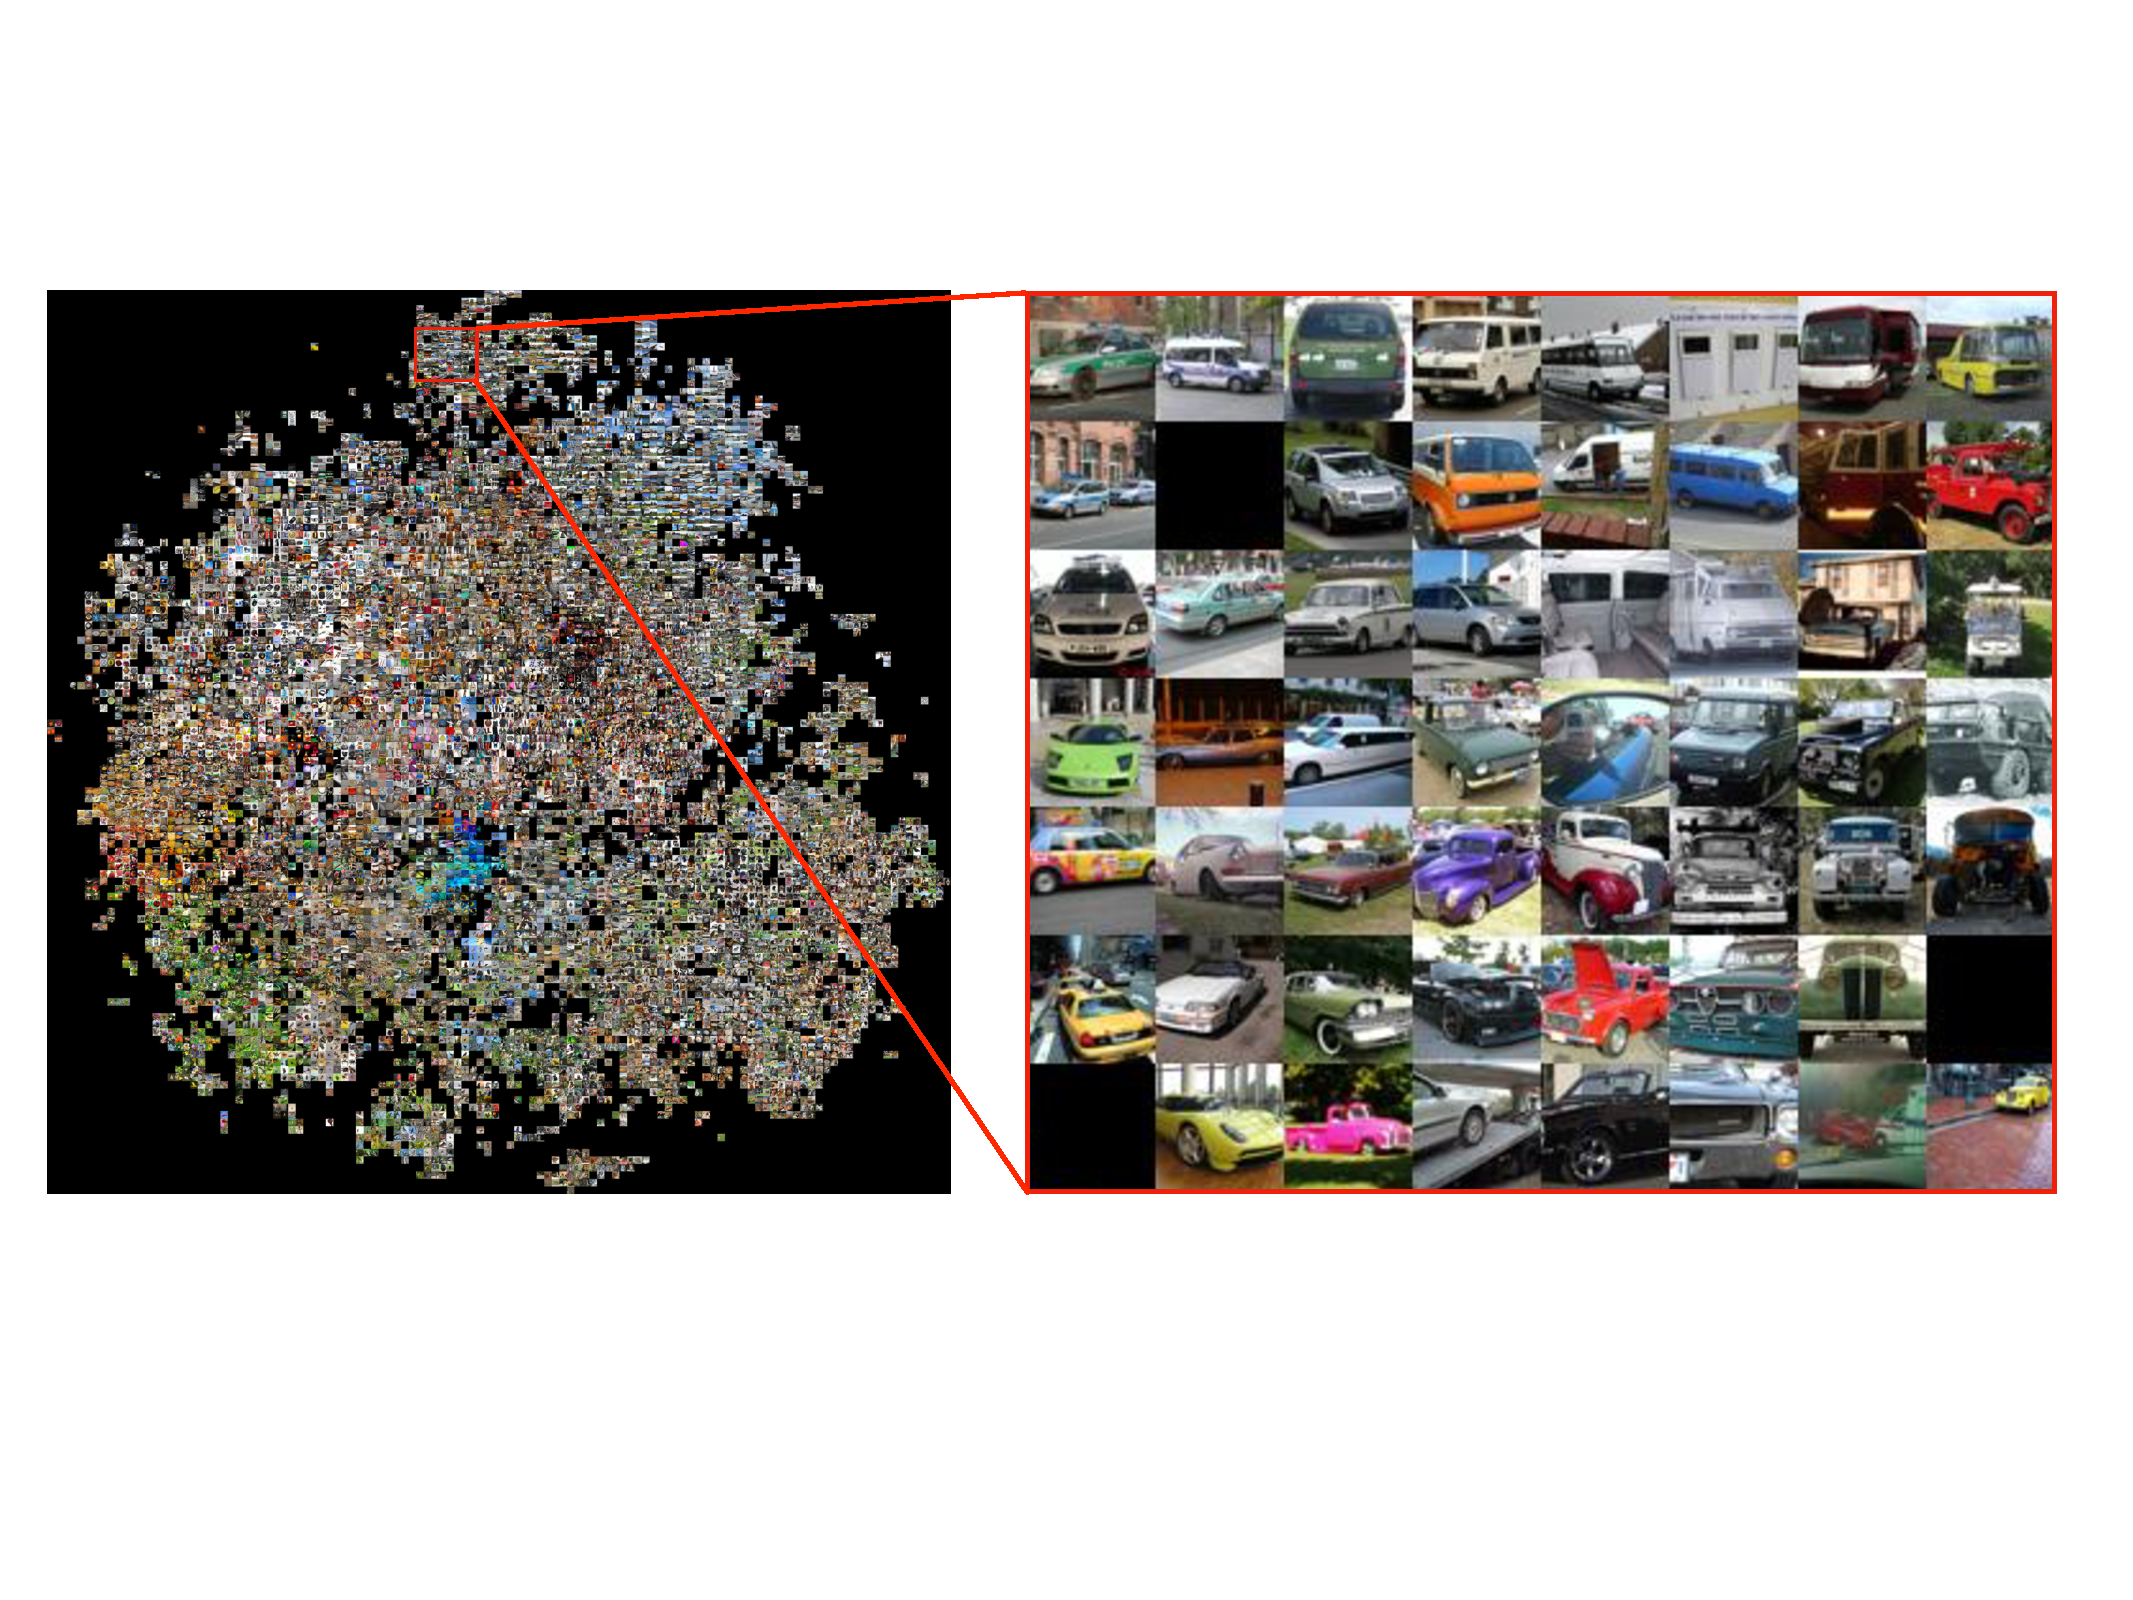
\includegraphics[width=\textwidth]{Vis_tsne_imagenet1.pdf}
%  \source{adapted from \url{https://cs.stanford.edu/people/karpathy/cnnembed/}}
\end{figure}
\end{frame}

\begin{frame}
\frametitle{t-SNE map: ImageNet}
\begin{figure}[htb]
  \centering
  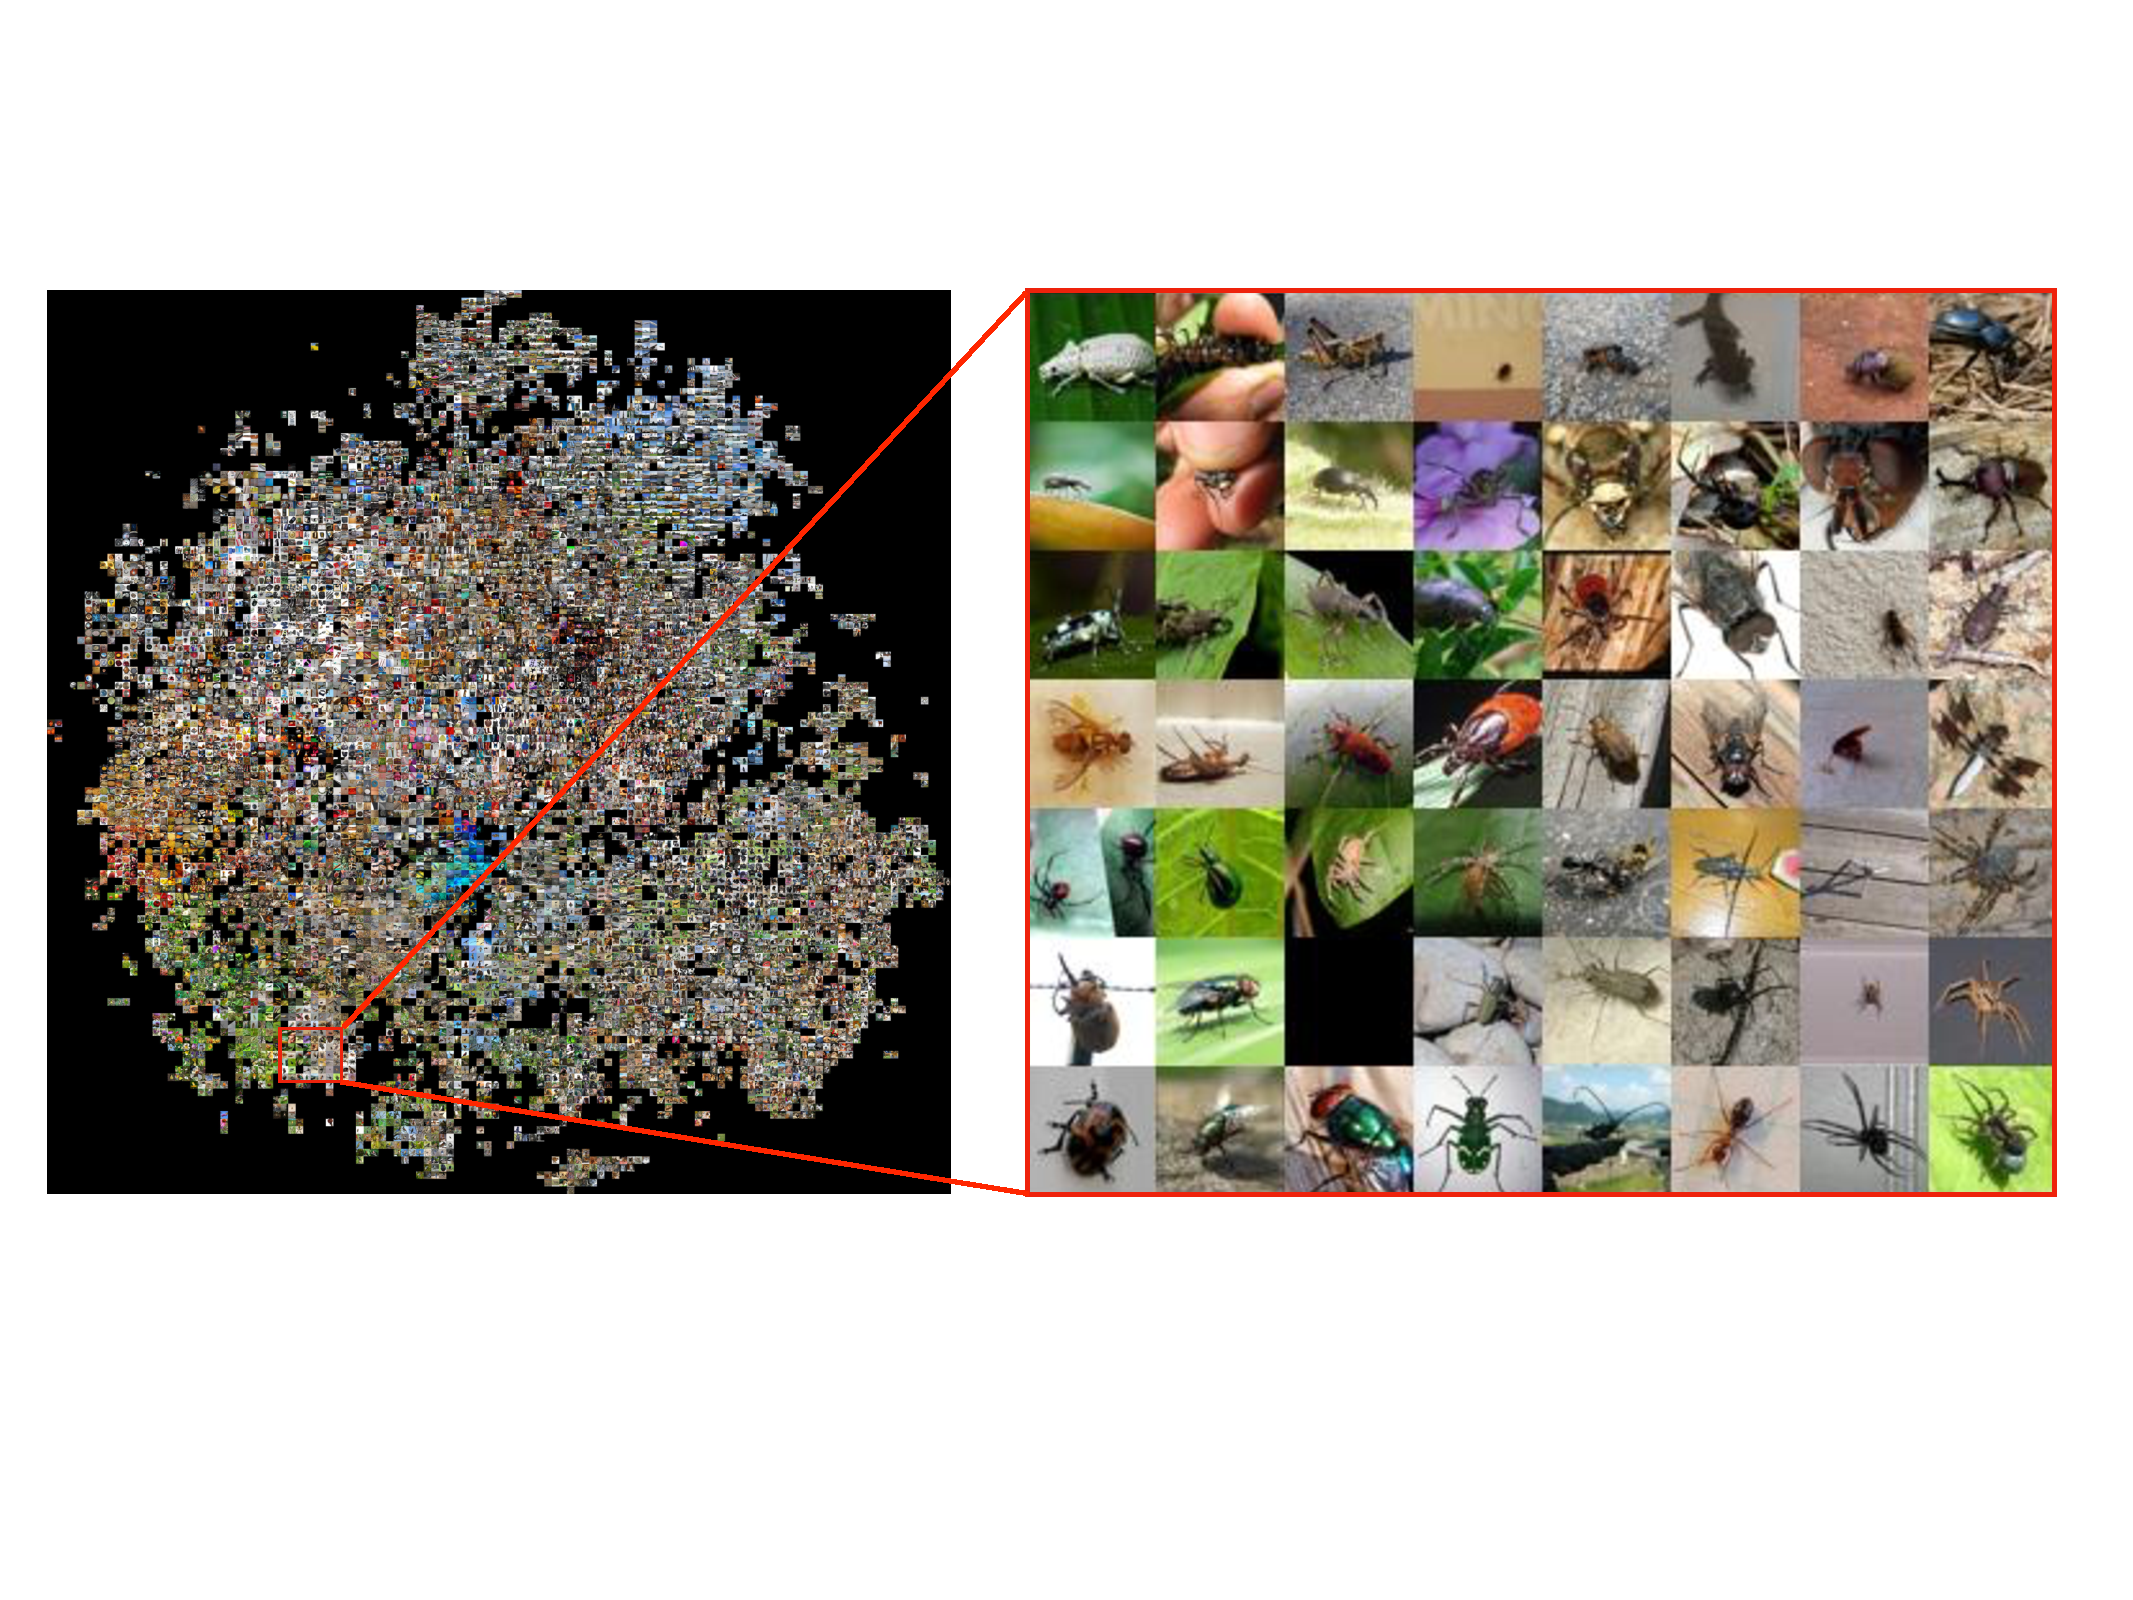
\includegraphics[width=\textwidth]{Vis_tsne_imagenet2.pdf}
%  \source{adapted from \url{https://cs.stanford.edu/people/karpathy/cnnembed/}}
\end{figure}
\end{frame}

\begin{frame}
\frametitle{t-SNE map: ImageNet}
\begin{figure}[htb]
  \centering
  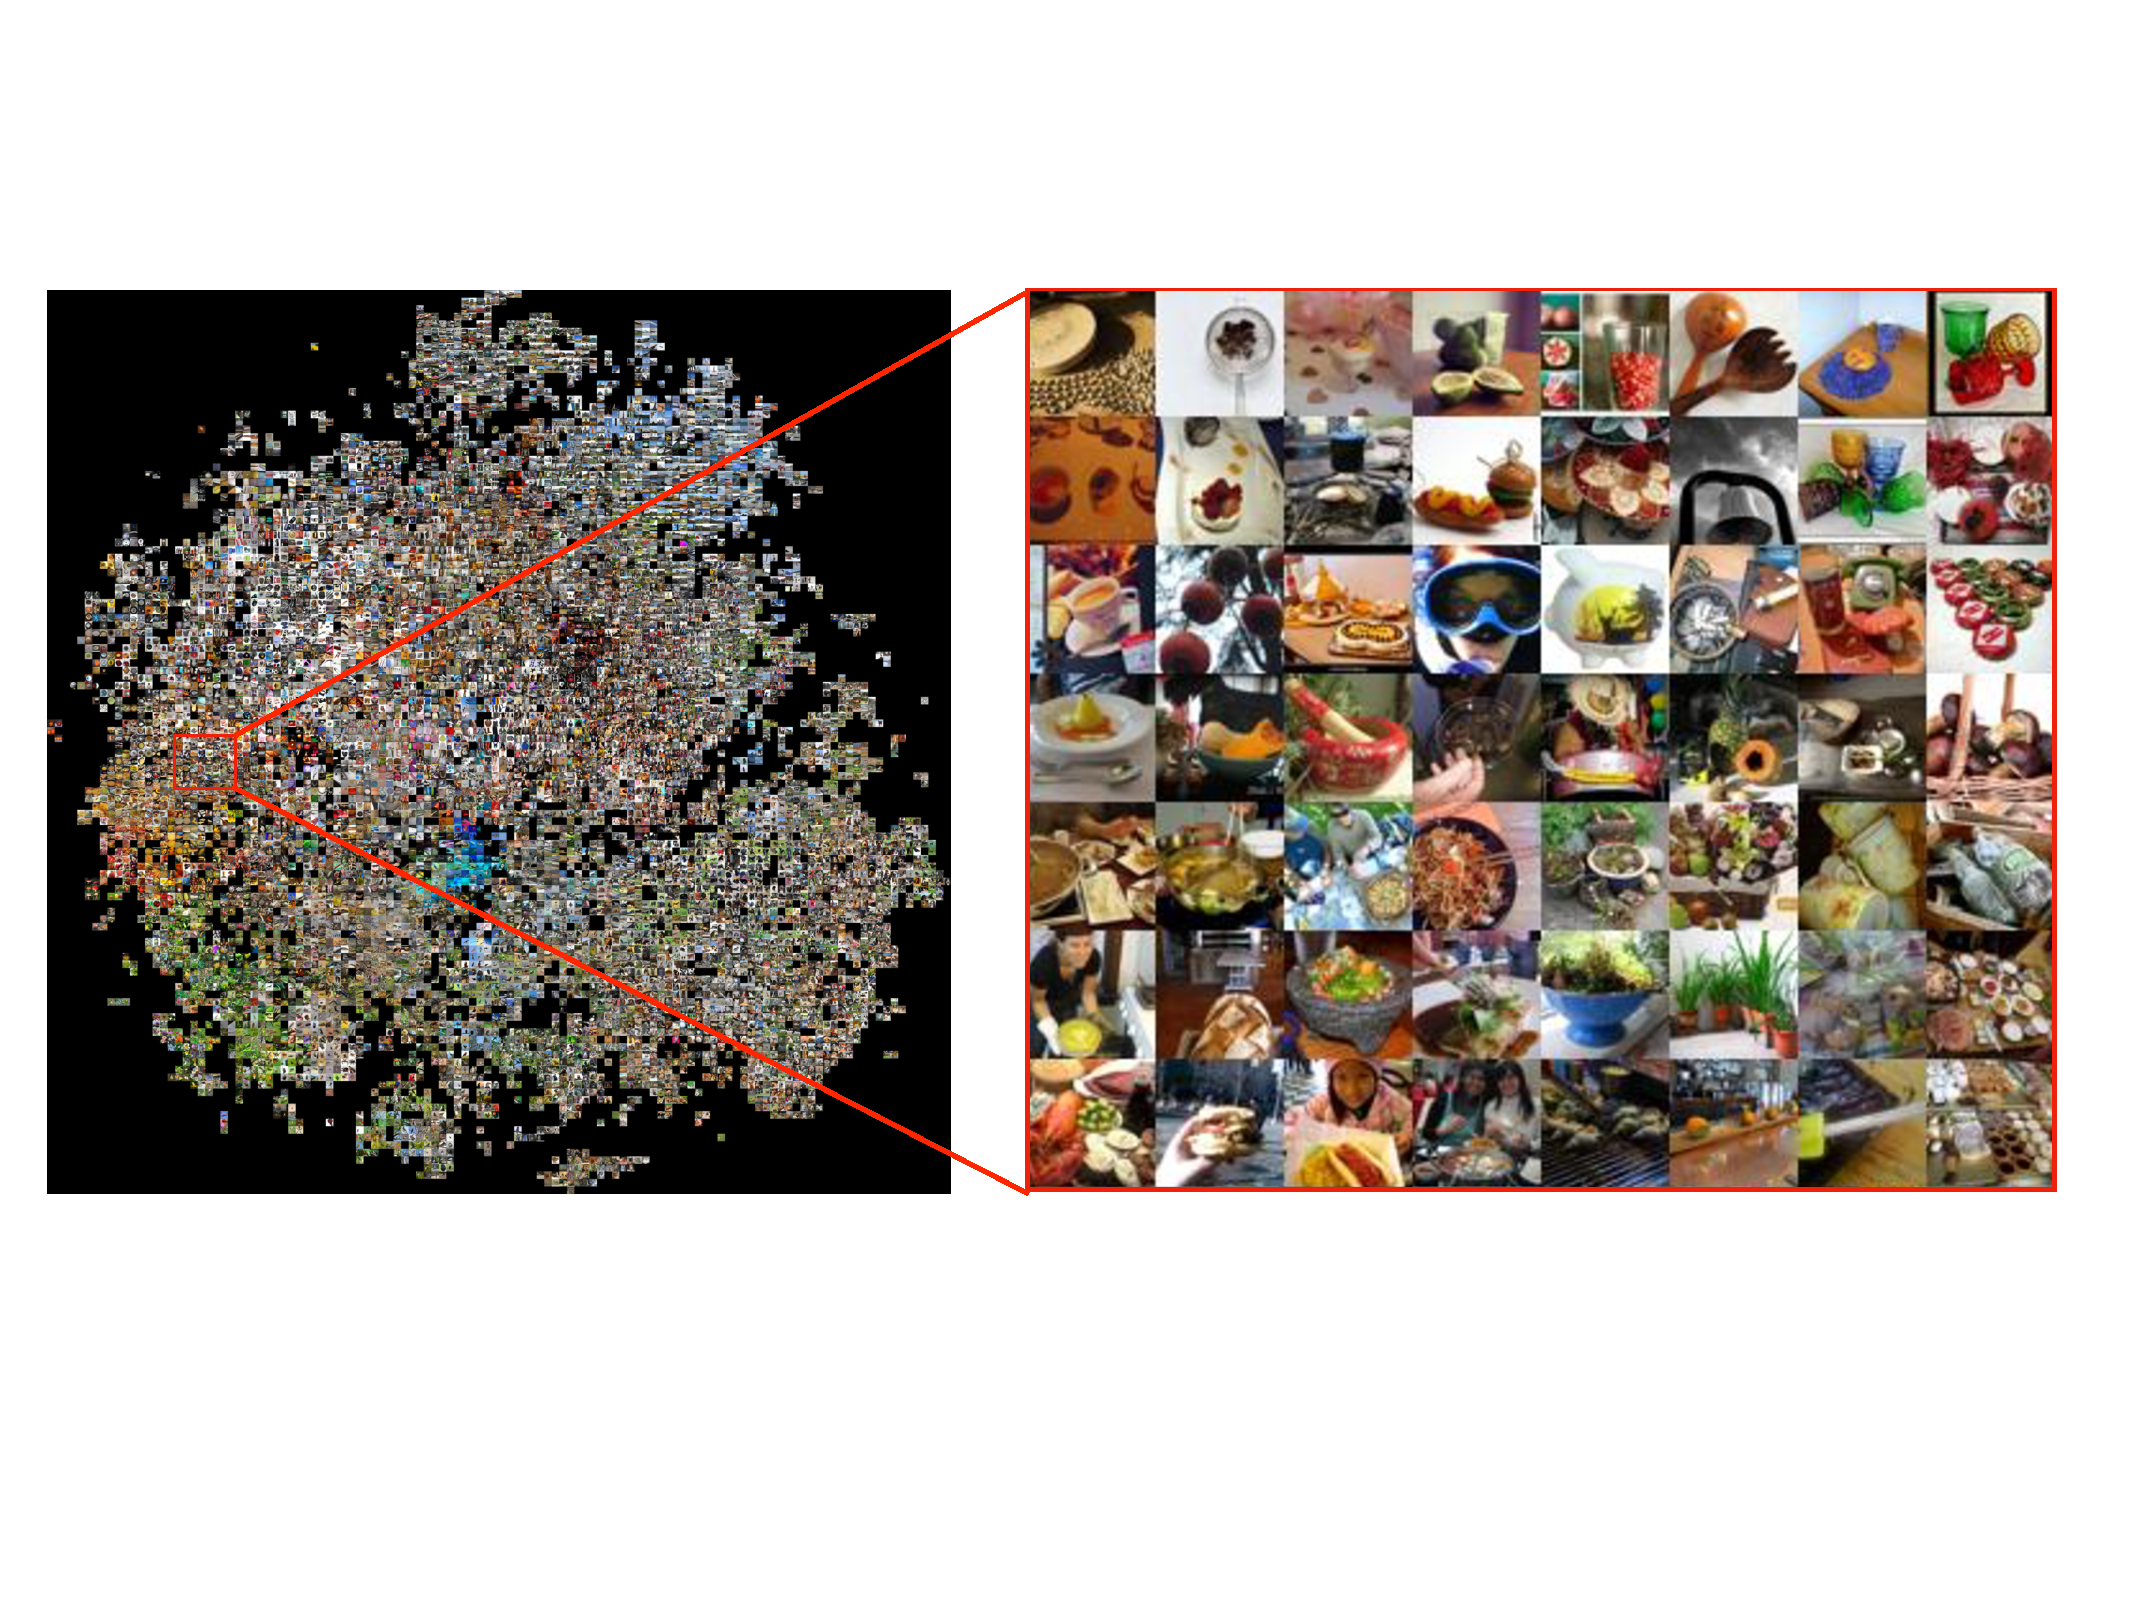
\includegraphics[width=\textwidth]{Vis_tsne_imagenet3.pdf}
%  \source{adapted from \url{https://cs.stanford.edu/people/karpathy/cnnembed/}}
\end{figure}
\end{frame}

\begin{frame}
\frametitle{Conclusion}
\begin{itemize}
	\item Méthodes de sélection par filtrage ad-hoc
	\item Méthodes de conteneur : sélection de variables pour une classification spécifique
	\item Méthodes embarquées (LASSO, ... )
	\item APC : analyse en composante principale
	\item t-SNE : méthode utilisée pour la visualisation. 
\end{itemize}
\end{frame}


